\chapter{State of the Art}
\label{cap:state-of-the-art}

This chapter presents the state of the art approaches for addressing the
issues presented in the previous chapter. The first part is characterized
by the analysis of Checkpoint/Restart techniques available in literature,
with a particular focus on HPC environments and MPI
applications.
The second part instead aims at providing an overview of solutions to perform
\emph{process migration},
including the migration of MPI processes. Finally the chapter is closed by a
brief survey of distributed resource management approaches.

\section{Checkpoint/Restart approach}
\label{sec:CRApproach}

\begin{figure}[t]
		\centerline 
{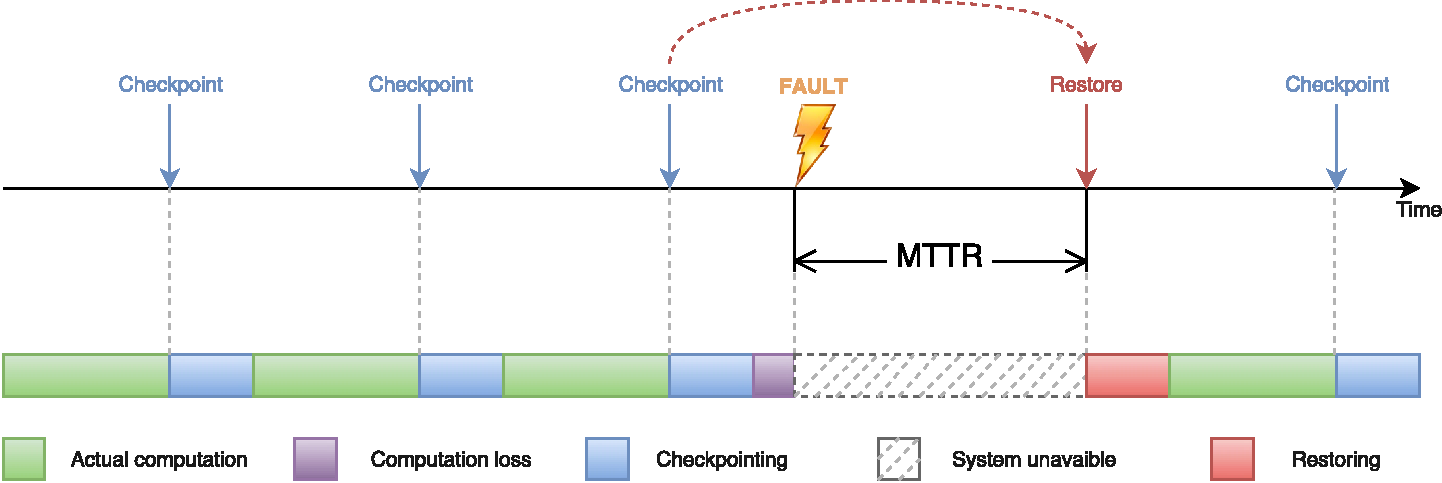
\includegraphics[scale=0.55]{img/cap2-cr.pdf}}
		\caption[The Checkpoint/Restart approach]{The Checkpoint/Restart approach.}
		\label{fig:checkpointrestore}
\end{figure}

\textbf{Checkpoint/Restart (C/R)} -- sometimes called Checkpoint/Restore -- is a \linebreak
widespread technique to enforce fault tolerance in computing systems. C/R are
essential for parallel and in particular HPC applications for the reason
presented in Chapter \ref{cap:introduction}.
C/R tools perform periodical \emph{checkpoint}s to save the state of the 
processes in a persistent storage medium. This state is usually called \emph{image}.
After a system fault, the image can be recovered in
order to \emph{restart} the execution from the saved checkpoint state. The
idea is depicted in Figure \ref{fig:checkpointrestore}.
C/R tools usually adopt the following schema:
\begin{enumerate}
\item Synchronization of the application processes execution to
reach a global consistent state;
\item Application execution state saving (\emph{checkpoint}); 
\item Application execution resuming (\emph{restart}).
\end{enumerate}
In case of fault of parallel applications, all the running processes
are killed and the application is restarted resuming the state from the last
checkpoint. Fault-tolerance approaches like C/R are called
\textbf{Rollback-recovery techniques} \cite{elnozahy2002survey}.

\subsection{Classification}
At first glance, we can classify
Checkpoint/Restart approaches on the basis of the level at which they operate:

\begin{itemize}
	\item \textbf{Application-level}: the C/R functionalities are provided by
	a specific library linked with the application. Usually the
	application is aware of C/R and must provide barriers or similar
	synchronization point to reach a consistent state of all
	processes and threads. Reaching a so called
	\textbf{Global Consistent State} allows the
	library to perform a safe checkpoint and restore;
	\item \textbf{System-level}: the C/R is performed by the operating
	system or by the programming framework (e.g. MPI). The application 
	is usually unaware of C/R and cannot therefore handle C/R events.
\end{itemize}

Alternatively, we can distinguish C/R approaches on the basis of the software
layer, or granularity, at which they act:

\begin{itemize}
	\item \textbf{Virtual Machine-level}: the classic approach in
	Infrastracture-as-a-Service virtualization. The application
	processes are distributed in several virtual machines governed by
	a hypervisor. It provides the virtual machine requirements
	(e.g. isolation) and also the capability of C/R (called 
	\emph{snapshots}). A
	virtual machine can be moved to another physical server or stopped
	and resumed if needed;
	\item \textbf{Container-level}: the operating system-level
	virtualization provides \emph{containers} on top of which the application
	processes run in a isolated environment. The approach is similar to
	the one based on virtual machines with the exception that there is only one
    instance of guest OS running on the host machine.
	Similarly to Virtual Machines, the C/R tools for containers
	are usually available and easy to implement and use;
	\item \textbf{Process-level}: C/R saves and restores the execution of each
    single process.
	This approach is more complex than moving a virtual machine or a
	container because the process is not completely isolated, In fact, in order
    to correctly save the execution status,
	all the input/output channels (file descriptor, sockets,
	etc.) need to be closed. The restore stage also presents several problems,
    for instance when the execution is resumed, the process identification number
    (PID) must be guaranteed to be the same. However, running
	natively the application on the system does not add the typical
	overhead of virtual machines and containers.
\end{itemize}


As shown by the timeline in Figure \ref{fig:checkpointrestore}, the cost of
C/R is very high in terms of wasted time, especially, due to the periodic
checkpoints required. Consequently, the overall overhead may reach over the
50\% \cite{fiala2012detection} of the total execution time.


\subsection{Libraries and frameworks}
The scientific interest in Checkpoint/Restart started in early 1990s with
some \emph{application-level} libraries. The first approaches to
\emph{system-level} checkpoints \linebreak started in the same years, however the
\emph{system-level} tools most used today were created after 2005.

Regarding the application-level mechanism, one of the most known libraries is
\texttt{libckpt} developed in 1994 by University of Tennessee for UNIX systems
and later ported to Linux \cite{plank1994libckpt}.
The user application has to be modified by adding the \texttt{libckpt}
function calls, in order to instruct the linked library to periodically
perform the checkpoints (default interval 10 minutes).
This library implements also \emph{incremental checkpoints}, that instead
of create and save a full image for every checkpoint, it stores only the
difference between the last and the current state images. With incremental
checkpoints the overall size of subsequent images on disk is dramatically
reduced and consequently it also limits the I/O overhead due to the image
storing.

In 2003 the Department of Computer Science of the Berkeley Laboratory (US
Department of Energy) developed the \textbf{Berkeley Lab Checkpoint/Restart
(BLCR)} software \cite{hargrove2006berkeley}. The approach is a process-level
C/R for Linux, with a hybrid kernel/user space implementation, designed with
HPC applications in mind. This open source tool was improved and maintained
until 2013. BLCR requires to load a custom kernel module, that is in charge of
providing the access to data usually neither visible nor modifiable from
user-space.
For instance, the possibility to alter the PID sequence or to know the filename
associated to one file descriptor. The user-space BLCR software uses the API
provided by the kernel module to implement the checkpoint and the restart
of the process.

Starting from Linux version 3.3 (released on March 18, 2012), it became
possible to produce full user-space C/R tool, thanks to the

\lstdefinestyle{customkernelopt}{
  belowcaptionskip=1\baselineskip,
  breaklines=true,
  frame=l,
  xleftmargin=\parindent,
  language=C,
  basicstyle=\footnotesize\ttfamily
}

\lstset{%
}%
\begin{lstlisting}[style=customkernelopt]
CONFIG_CHECKPOINT_RESTORE
\end{lstlisting}

kernel option. This option enables
the application to access to kernel parameters, like modify the next PID in the
PID sequence. To the best of our knowledge, \textbf{CRIU (Checkpoint/Restore
in Userspace)} \cite{CRIU} is currently the only available tool that exploits
that kernel option. Since an user-space tool presents several advantages
(higher portability, security, maintainability, etc.) compared to a kernel-space one, CRIU was selected as C/R
tool for this thesis.
In the next chapter, a description of CRIU and the motivations of this choice
will be extensively discussed.

\subsection{Checkpoint/Restart in MPI}
Since the early years of development of MPI implementations, C/R was one of
the most hot research topic. Several C/R tools have been proposed to
be integrated in MPI framework or designed to directly work with MPI, like the
previously cited BLCR.

One of the first C/R implementations for MPI was proposed in 1997 by
\emph{Li et al.}
\cite{li1997checkpointing}. This C/R consists of multicast daemons that
assist the MPI runtime to perform communications and checkpoints. The
checkpoints are locally coordinated at single node level, while the processes
running on remote nodes are considered out of scope. Moreover, the multicast
daemons replace the MPI library communication module
in order to provide a retransmission mechanism
when messages are lost due to an ongoing checkpoint. This C/R was implemented
in the LAM/MPI library.

\emph{Hursey et al.} \cite{hursey2009interconnect} extended the Open MPI
stack with additional layers providing C/R capabilities. The approach is
based on a dedicated Checkpoint/Restart Coordination Protocol (CRCP), to
support the synchronization among the nodes of the distributed systems. The
coordination is split
is three phases: \linebreak \emph{pre-checkpoint}, \emph{continue} and \emph{restart}.
The first phase has the duty to bring the system to a checkpointable state,
i.e. it has to ensure the synchronization of the processes, the absence of
in-flight messages, a safe state of all file descriptors, etc. The
\emph{continue} phase is indeed the checkpoint: close all socket connections
and call the
BLCR routines in order to save the image. Finally, the \emph{restart} occurs
on demand (e.g. after a fault-recover) and restores the previously saved
image. A similar approach, still exploiting, BLCR was proposed in 2005
for LAM/MPI \cite{sankaran2005lam}.

One of the advantages of this technique is the ability to be network
agnostic. The application processes can be stopped
and then restarted on a different set of nodes, potentially
characterized by a different network topology. The coordination protocol has
to consider also the exchange of information about the new topology over all
nodes and their processes. However, this solution introduces noticeable code dependencies between internal
Open MPI modules. Moreover, it induces significant overheads: copying the
process state images onto an external storage server becomes in fact a real
bottleneck for the system. The previous drawbacks, along with the poor maintainability of the software,
led the Open MPI developers to disable these additional layers since Open MPI
version 1.7. Nevertheless, this work is still the only working C/R available in
the Open MPI mainline code repository.

For the sake of completeness, C/R can be used also for purposes different from
fault-tolerant. For example, it can be used to efficiently debug
parallel applications \cite{hursey2010checkpoint}: if the programmer want to
\emph{rewind} the execution,
he or she does not necessarily restart the application from the begin, but only
from the last saved checkpoint.

% ADD: http://ieeexplore.ieee.org/xpls/abs_all.jsp?arnumber=640140

\subsection{Limitations}
As already briefly discussed in Chapter \ref{cap:introduction}, the common
limitation of C/R based approaches is the overhead introduced by performing
periodical checkpoints, which is done during the entire application
lifespan. In some use cases this overhead impacts dramatically, even doubling
the execution time of the applications \cite{philp2005software}. For example,
to quantify this overhead, consider that in 2013 some TOP500 HPC systems
requires a checkpoint time between 40 to 60 minutes
\cite{egwutuoha2013survey}. A further problem is that this side-effect
increases exponentially with the system size, i.e. the number of computing
nodes. Considering a large HPC system with thousands of nodes and not
negligible power supply costs, the overhead must be evaluated not only in
terms of time, but also in terms of energy consumption
\cite{mills2013evaluating}.

In systems based on Virtual Machines or Containers, implementing C/R
mechanisms - even if
in conjunction with MPI - is relatively easy. However, virtual machines
also have a significant impact on the application performance, especially for 
I/O intensive workloads in HPC systems \cite{xavier2013performance}. The lack
of shared memory communication between processes on different virtual machines
indeed has been considered an important inefficiency since the
beginning of virtualization's use in HPC environments \cite{huang2007virtual}.
Although many approaches have been proposed to mitigate
this problem, the significant overhead persists even today,
inducing an increment of latency by a factor up to 16x for
communication intensive operations \cite{pickartz2016impacts}.

\section{Process migration in MPI}
\textbf{Process migration} - or \textbf{task migration} - is a technique that
can be used in alternative or in support to C/R. When the allocation of
nodes has to be changed (e.g. due to a failure of one node), classic C/R 
techniques consist in checkpoint the application a restart it over a different
subset of nodes. This job can be performed more efficiently with process
migration, in order to involve only the nodes that have to be moved.

In large cluster, process migration is useful to add reliability and
to balance the resource allocation across the cluster \cite{hussain2013survey}.
The migration request can be done centralized (e.g. by a resource manager) or
by the single node, that for instance may request a migration if it's overloaded
or an imminent fault is going to occur.
While it has the potential benefits described, the entity that triggers the
migration must take in account the considerable migration cost. 

In 1996, \emph{Stellner} proposed the first migration technique in MPI:
the \emph{Cocheck} environment \cite{stellner1996cocheck}. This environment
was built on top the MPI framework and not inside (actually small modifications
to MPI framework were applied). The global
consistent state is achieved by imposing no message in-flight over the
network. Then, checkpoint or a migration of a subset of processes is performed
according to what is required.

Process migration can be used also to supported classical C/R approaches, as
presented by \emph{Wang et al.} \cite{wang2008proactive}. Their work introduced
a process-level migration that allows us to potentially achieve a higher
utilization of the system resources, with respect to virtualization based
approach. The basic idea of the authors is to try to minimize the number of
C/R by using
a proactive approach: health monitoring of the computing node state and
migration of all the running processes on a different node, in case of
imminent fault prediction. Their approach reduces the number of performed C/R
with respect to periodical checkpoint based techniques. However this solution
requires to synchronize all the running processes into a global consistent
state, before stopping and migrating them to a new node. This can represent
an issue in case of imminent faults that require short time to act. The
approach was implemented in LAM/MPI (predecessor of Open MPI) using the BLCR
tool.

According to the aforementioned works, we can argue that the main
issues to be tackled when dealing with processes migration in HPC systems are:
\begin{itemize}
\item Design an easy to maintain migration framework;
\item Enable migration support without introducing changes in the application
code;
\item Enable the possibility of migrating just part of the application, i.e. a
subset of processes;
\item Do not bind the migration overhead to the synchronization of the
processes execution into a global consistent state;
\item Provide interfaces to allow a resource manager to drive the processes
migration according to smart policies.
\end{itemize}

The solution we propose addresses all the aforementioned issues:
\begin{enumerate}
\item It is a process-level migration mechanism whose granularity can be tuned by the resource manager;
\item It does not require any change to the application code;
\item The migration is almost completely transparent with respect to the
application execution;
\item Migration can be triggered by a resource manager through a suitable API.
\end{enumerate}

\subsection{Heterogeneous process migration}
Process migration is usually available in homogeneous 
clusters, since migration in heterogeneity conditions is much more complex
\cite{hussain2013survey}.

In 1998, \emph{Smith et al.} presented the Tui System
\cite{smith1998heterogeneous}, an experimental framework to perform process
migration between heterogeneous machines. The article was well received by
the scientific community and it shows the several issues affecting the
heterogeneous migration. The main problem is the conversion between different
ISA, that may require different instructions, register numbers, register size,
etc. For this reason, the compiler is compulsory involved, because it must
produce a code that matches one-to-one between different architecture.
As a consequence, in order to simplify the problem, the Tui System has strong
constraints regarding the two architectures involved, that leads to a
migration much more \emph{quasi-homogeneous} than heterogeneous.

Other few solutions were proposed, e.g. \emph{Cabello et al.}
\cite{cabello2014fault}
proposed an Open MPI middleware to provide migration mechanism
in heterogeneous systems. In this case the process is not directly migrated
but a new process is started in the destination machine. Unfortunately, this
middleware provides dedicated MPI calls, violating the standard and requiring
substantial rewrite of all MPI applications.

\section{Distributed resource management}
The academic interest in resource management significantly increased
since 2005,
when the first multi-core processors became available. However, the resource
management of distributed systems goes back to 90s, when the resource
scheduling and allocation became a necessity for large data-centers. 

Classical feature of a resource management systems is to provide an efficient
assignment of resources to jobs. This problem is called \textbf{resource
allocation} or \textbf{resource scheduling} \cite{raman1998matchmaking}.

For the first Grid systems\footnote{A Grid system is a large distributed
Network Computing system with machines distributed over several data-centers}
resource management was essential and still plays a crucial role in this type
of distributed systems. The resource manager has to cooperate to guarantee
the properties
of scalability, responsiveness, fault-tolerance, stability - that are in 
common with Distributed Computing Environments - but also security,
heterogeneity, isolation, distributed ownership, and QoS
\cite{krauter2002taxonomy}. In this regard, a variant of MPICH
- called MPICH-G - was proposed in 1998 to enable MPI to work in Grid computing
\cite{foster1998grid}.

Nowadays, delivering high throughput and low latency in supercomputers getting
close to Exascale requires a resource management system sufficiently
scalable. Current centralized resource managers seem not a feasible solution
to guarantee the performance requirements in Exascale, so the current
research is oriented in distributed resource management \cite{wang2014next}.

Not all HPC environments require a perfect efficient scheduling of resources,
due to policy reasons. In distributively owned environments, the owner of
a resource defines the access policy for that specific resource, for
instance setting
time constraints. These policies introduce more complexity in modeling
the system, and consequently in the resource management performance
\cite{raman1998matchmaking}.

Furthermore, in last years, distributed resource management becomes not only
important for HPC applications, but also for energy-aware resource management
in Cloud Computing infrastructures \cite{beloglazov2012energy}. 

\subsection{Resource Management and Open MPI}
\begin{table}[ht!b]
\centering
\begin{tabular}{ c|c|c|c}

\textbf{Name} 
& 
\parbox{4.5cm}{\vspace{.5\baselineskip}
\centering \textbf{Developer} 
\vspace{.5\baselineskip}}
& \textbf{Last stable release} 
& \textbf{Reference} \\ \hline

ALPS 
& 
\parbox{4cm}{\vspace{.5\baselineskip}
\centering Cray User Group 
\vspace{.5\baselineskip}}
& April, 2012
& \cite{karo2006application}
\\ \hline

Grid Engine
&  
\parbox{4.5cm}{\vspace{.5\baselineskip}
\centering Proprietary and open source implementations available 
 \vspace{.5\baselineskip}}
&
\parbox{3cm}{\vspace{.5\baselineskip}
\centering  January, 2014 (open source version)
 \vspace{.5\baselineskip}}
& \cite{gentzsch2001sun}
\\ \hline

LoadLeveler
& 
\parbox{4cm}{\vspace{.5\baselineskip}
\centering IBM Corporation 
\vspace{.5\baselineskip}}
& unknown
& N.A.
\\ \hline

LSF
& 
\parbox{4cm}{\vspace{.5\baselineskip}
\centering IBM Corporation 
\vspace{.5\baselineskip}}
& August, 2016
& \cite{zhou1992lsf}
\\ \hline

SLURM
& 
\parbox{4cm}{\vspace{.5\baselineskip}
\centering Open Source community
\vspace{.5\baselineskip}}
& July, 2016
& \cite{yoo2003slurm}
\\ \hline

Torque (ex PBS)
& 
\parbox{4cm}{\vspace{.5\baselineskip}
\centering Adaptive Computing
\vspace{.5\baselineskip}}
& August, 2016
& \cite{staples2006torque}

\end{tabular}

\caption[Supported resource managers in Open MPI]{The supported resource managers in Open MPI.}
\label{tab:rmopenmpi}

\end{table}

At the time of writing Open MPI supports several resource managers, as
summarized in Table \ref{tab:rmopenmpi}. Most of them statically assign the
resource
to the MPI application at launch-time. Two different approaches are used in
current resource managers: interactive or wrapped. In the first case, the
\texttt{mpirun} command is invoked while Open MPI subsequently 
interrogates the resource manager asking to which nodes dispatch the application processes. 
In the second case, a wrapper script
interrogates the resource manager and subsequently execute the
\texttt{mpirun} command. Then, Open MPI typically retrieves the information
via environment variables or similar mechanisms.

Even if some of the previous resource managers offers features like C/R
and migration (e.g. SLURM via BLCR), they are not integrated in Open MPI.
The first part of our work is to add the support of the BarbequeRTRM to
Open MPI, including the dynamic rescheduling of application during runtime.
This feature is implemented with process migration.
